%!TEX root = Reader.tex
\part{Module 2: Probability Fundamentals}

% --- Lecture 3 ---
%\begin{frame}{Lecture 3: Rules of Probability}
%    \small
%    \begin{itemize}
%        \item \textbf{15 mins:} Definitions \& Notation.
%            \begin{itemize}
%                \item Sample Space ($S$), Events, Complement ($P(A') = 1 - P(A)$).
%                \item \textit{Cut: Classical vs. Empirical (Assign as reading).}
%            \end{itemize}
%        \item \textbf{20 mins:} The Addition Law (Unions).
%            \begin{itemize}
%                \item Mutually Exclusive: $P(A \cup B) = P(A) + P(B)$.
%                \item General Rule: $P(A \cup B) = P(A) + P(B) - P(A \cap B)$.
%            \end{itemize}
%        \item \textbf{15 mins:} The Multiplication Law (Intersections).
%            \begin{itemize}
%                \item Independent Events: $P(A \cap B) = P(A) \times P(B)$.
%                \item Conditional Probability: $P(A \cap B) = P(A) \times P(B|A)$.
%            \end{itemize}
%    \end{itemize}
%\end{frame}

\section{Probability Fundamentals}

\only<article>{
    Welcome to Module 2. In the previous module, we learned how to mathematically describe data that we have already collected (the past). Now, we shift our focus to predicting the likelihood of events before they happen (the future). 
    
    Probability forms the absolute mathematical foundation of risk assessment, reliability engineering, signal processing, and system design. In this lecture, we will establish the fundamental rules and notation that govern random events.
}

\section{Outline of next part}
% --- Lecture 3 Outline ---
\begin{frame}{Outline}

    
    \begin{itemize}
        \item \textbf{Definitions \& Notation}
            \begin{itemize}
                \item Sample Space ($S$), Events, Complement ($P(A') = 1 - P(A)$).
            \end{itemize}
            
        \only<presentation>{\vspace{0.3cm}}
            
        \item \textbf{The Addition Law (Unions)}
            \begin{itemize}
                \item Mutually Exclusive: $P(A \cup B) = P(A) + P(B)$.
                \item General Rule: $P(A \cup B) = P(A) + P(B) - P(A \cap B)$.
            \end{itemize}
            
        \only<presentation>{\vspace{0.3cm}}
            
        \item \textbf{The Multiplication Law (Intersections)}
            \begin{itemize}
                \item Independent Events: $P(A \cap B) = P(A) \times P(B)$.
                \item Conditional Probability: $P(A \cap B) = P(A) \times P(B|A)$.
            \end{itemize}
    \end{itemize}
    
    \only<article>{
        \vspace{0.3cm}
        \textit{Pre-reading Note: Students are expected to review the difference between \textbf{Classical} (theoretical) and \textbf{Empirical} (observational) probability in the course textbook prior to engaging with this material.}
    }
\end{frame}

\section{Probability Fundamentals}



\only<article>{
    Welcome to Module 2. In the previous module, we learned how to mathematically describe data that we have already collected (the past). Now, we shift our focus to predicting the likelihood of events before they happen (the future). 
    
    Probability forms the absolute mathematical foundation of risk assessment, reliability engineering, signal processing, and system design. In this lecture, we will establish the fundamental rules and notation that govern random events.
}

% --- Lecture 3 Outline ---
\begin{frame}
\frametitle{Outline}
    \only<article>{
        \textbf{Lecture Outline:}
    }
    
    \begin{itemize}
        \item \textbf{Definitions \& Notation}
            \begin{itemize}
                \item Sample Space ($S$), Events, Complement ($P(A') = 1 - P(A)$).
            \end{itemize}
            
        \only<presentation>{\vspace{0.3cm}}
            
        \item \textbf{The Addition Law (Unions)}
            \begin{itemize}
                \item Mutually Exclusive: $P(A \cup B) = P(A) + P(B)$.
                \item General Rule: $P(A \cup B) = P(A) + P(B) - P(A \cap B)$.
            \end{itemize}
            
        \only<presentation>{\vspace{0.3cm}}
            
        \item \textbf{The Multiplication Law (Intersections)}
            \begin{itemize}
                \item Independent Events: $P(A \cap B) = P(A) \times P(B)$.
                \item Conditional Probability: $P(A \cap B) = P(A) \times P(B|A)$.
            \end{itemize}
    \end{itemize}
    
    \only<article>{
        \vspace{0.3cm}
        \textit{Pre-reading Note: Students are expected to review the difference between \textbf{Classical} (theoretical) and \textbf{Empirical} (observational) probability in the course textbook prior to engaging with this material.}
    }
\end{frame}

% -----------------------------------------------------------------------------
% Lecture 3: Rules of Probability
% -----------------------------------------------------------------------------
\subsection{Definitions \& Notation}

\begin{frame}[allowframebreaks]{The Sample Space and Events}
    \begin{definition}[Experiment and Sample Space]
        An \textbf{experiment} is any process whose outcome is subject to uncertainty. \\
        The \textbf{sample space} ($S$) is the set of all possible outcomes.
    \end{definition}

    \only<article>{
        In your previous math classes, probability experiments usually involved rolling dice or drawing playing cards. In engineering, an experiment is a quality assurance test, a sensor reading, or a system failure check.
    }

    \begin{example}[Testing Microcontrollers]
        Suppose we test 3 microcontrollers off a production line. Each either Passes ($P$) or Fails ($F$). 
        The sample space has 8 possible outcomes:
        \[ S = \{PPP, PPF, PFP, PFF, FPP, FPF, FFP, FFF\} \]
    \end{example}

    \begin{definition}[Event]
        An \textbf{event} is any subset of the sample space. 
    \end{definition}
    
    \only<presentation>{\vspace{0.2cm}}
    
    If we define Event $A$ as \lq exactly one microcontroller fails\rq, then:
    \[ A = \{PPF, PFP, FPP\} \]
\end{frame}

\begin{frame}{Set Operations in Probability}
    Events are usually combined using standard set operations. Let $A$ and $B$ be events in sample space $S$.

    \begin{itemize}
        \item \textbf{Complement ($\bar{A}$ or $A'$):} All outcomes \textit{not} in $A$. 
        \begin{itemize}
            \item $P(\bar{A}) = 1 - P(A)$
        \end{itemize}
        \item \textbf{Intersection ($A \cap B$):} Outcomes in both $A$ \textbf{AND} $B$.
        \item \textbf{Union ($A \cup B$):} Outcomes in $A$ \textbf{OR} $B$ (or both).
        \item \textbf{Mutually Exclusive ($A \cap B = \varnothing$):} Events that cannot happen at the same time. The intersection is the empty set ($\varnothing$).
    \end{itemize}

    \only<article>{
        
        
        \textbf{Visualising Probability:} Venn diagrams are the engineer's best friend for probability. The outer box represents the entire sample space $S$ (where total probability = $1$). The circles represent events. If the circles overlap, the events can happen simultaneously (Intersection). If they don't overlap, they are mutually exclusive.
    }
\end{frame}

% -----------------------------------------------------------------------------
\subsection{The Addition Law}

\begin{frame}{The Addition Law (Unions)}
    How do we calculate the probability of $A$ \textbf{OR} $B$ happening?

    \begin{block}{1. For Mutually Exclusive Events}
        If $A$ and $B$ cannot happen together ($A \cap B = \varnothing$), we simply add their probabilities:
        \[ P(A \cup B) = P(A) + P(B) \]
    \end{block}

    \only<presentation>{\pause \vspace{0.2cm}}

    \begin{alertblock}{2. The General Addition Rule}
        If events \textit{can} happen together, simply adding them will count the intersection twice. We must subtract the overlap:
        \[ P(A \cup B) = P(A) + P(B) - P(A \cap B) \]
    \end{alertblock}

    \only<article>{
        \begin{example}[Manufacturing Defects]
            A batch of printed circuit boards (PCBs) is tested. 
            \begin{itemize}
                \item Event $A$: The board has a soldering defect ($P(A) = 0.10$).
                \item Event $B$: The board has a trace defect ($P(B) = 0.05$).
                \item Both defects: $P(A \cap B) = 0.02$.
            \end{itemize}
            What is the probability a board has \textit{at least one} defect ($A \cup B$)?
            \[ P(A \cup B) = 0.10 + 0.05 - 0.02 = \mathbf{0.13} \text{ (or 13\%)} \]
            If we hadn't subtracted the 2\% overlap, we would have mathematically rejected too many boards!
        \end{example}
    }
\end{frame}

% Requires \usepackage{tikz} and \usetikzlibrary{patterns} in your main file.

\begin{frame}{Visualising the Addition Law}
    The addition law: $P(A \cup B) = P(A) + P(B) - P(A \cap B)$. \\
    Venn diagrams make the subtraction intuitive.

    \centering
    \begin{tikzpicture}[scale=0.9, every node/.style={scale=0.9}]
        % Setup coordinates and definitions
        \def\r{1.5} % radius of the circles
        \coordinate (Acoord) at (-\r/2, 0);
        \coordinate (Bcoord) at (\r/2, 0);

        % --- Step 1: Base outlines (always visible) ---
        \draw[thick] (-3.5, -2) rectangle (3.5, 2.5); % Sample space S
        \node[anchor=north west] at (-3.5, 2.5) {$S$};
        \node[gray] at (-2, 1.8) {$P(S)=1$};

        \draw (Acoord) circle (\r);
        \draw (Bcoord) circle (\r);
        \node at (-2, 1) {$A$};
        \node at (2, 1) {$B$};

        % --- Step 2: Shade A (visible from slide 2 onwards) ---
        \only<2->{
            % Custom color for A from previous examples
            \fill[blue, opacity=0.3] (Acoord) circle (\r);
            % Instructor note (visible only in handout/article mode)
            \only<article>{Start with the entire area of Event A: $P(A)$.}
        }

        % --- Step 3: Shade B (visible on slide 3 and 4) ---
        \only<3-4>{
            % Custom color for B
            \fill[red, opacity=0.3] (Bcoord) circle (\r);
            
            % Highlight the intersection area showing it's darker
            \begin{scope}
                \clip (Acoord) circle (\r);
                \fill[purple, opacity=0.4] (Bcoord) circle (\r); % Darker overlap
            \end{scope}
            
            %Instructor note
            \only<article>{Add the entire area of Event B: $+P(B)$. The middle area turns purple because we have counted it twice!}
        }

        % --- Step 4: Visualise the overlap to subtract (slide 4) ---
        \only<4>{
            \draw[<-] (0,0) -- (1, -1.2) node[below] {\alert{Counted Twice!}};
        }

        % --- Step 5: Final Union (visible on slide 5) ---
        \only<5>{
            % Shading the exact union smoothly
            \begin{scope}
                \fill[purple!50!white] (Acoord) circle (\r);
                \fill[purple!50!white] (Bcoord) circle (\r);
            \end{scope}
            
            % Redraw outlines on top for sharpness
            \draw (Acoord) circle (\r);
            \draw (Bcoord) circle (\r);
            
            % Label intersection
            \draw[<-] (0,0) -- (0.8, -1.2) node[below] {$A \cap B$};
            \node at (0, 2) {\textbf{The Union} ($A \cup B$)};

            %Instructor note
            \only<article>{Subtract the intersection $- P(A \cap B)$. This leaves us with a smooth total area covered by A or B: $P(A \cup B)$.}
        }

    \end{tikzpicture}
    
    % --- Instruction Block (appearing at the end) ---
    \only<presentation>{
        \pause[5] \vspace{-2mm}
        \begin{block}{Why do we subtract?}
            Adding $P(A) + P(B)$ counts the intersection \textbf{twice}. To fix this, we must subtract one instance of the intersection:
            \[ P(A \cup B) = P(A) + P(B) - P(A \cap B) \]
        \end{block}
    }
\end{frame}

\begin{frame}{A Simple Dice Example}
    \begin{example}[The 6-Sided Die]
        Consider rolling a fair 6-sided die. Let event $A$ be rolling an even number, and let event $B$ be rolling a number divisible by 3.
        
        \structure{Questions:}
        \begin{enumerate}
            \item Write down the elements of subsets $A$ and $B$.
            \item Calculate $P(A)$ and $P(B)$.
            \item Write down the elements of the intersection (the event that the number is both even \textbf{and} divisible by 3) and calculate its probability, $P(A \cap B)$.
            \item Calculate the probability that the number rolled is either even \textbf{or} divisible by 3, $P(A \cup B)$, by counting the elements.
            \item Confirm the General Addition Law for this case.
            \item Are events $A$ and $B$ mutually exclusive?
        \end{enumerate}  
    \end{example}
\end{frame}


% --- Slide 1 of 3 ---
\begin{frame}{Solution: A Simple Dice Example (1/3)}
    \begin{solution}
        \textbf{1. Elements of $A$ and $B$:}
        \begin{itemize}
            \item Sample space $S = \{1, 2, 3, 4, 5, 6\}$
            \item $A$ (Even numbers) $= \{2, 4, 6\}$
            \item $B$ (Divisible by 3) $= \{3, 6\}$
        \end{itemize}
        
        \pause \vspace{0.4cm}
        
        \textbf{2. Calculate $P(A)$ and $P(B)$:}
        \begin{itemize}
            \item $P(A) = \frac{3}{6} = \frac{1}{2}$
            \item $P(B) = \frac{2}{6} = \frac{1}{3}$
        \end{itemize}
    \end{solution}
\end{frame}

% --- Slide 2 of 3 ---
\begin{frame}{Solution: A Simple Dice Example (2/3)}
    \begin{solution}
        \textbf{3. Intersection $P(A \cap B)$:}
        \begin{itemize}
            \item The only number both even \textbf{and} divisible by 3 is 6.
            \item $A \cap B = \{6\}$
            \item $P(A \cap B) = \frac{1}{6}$
        \end{itemize}

        \pause \vspace{0.4cm}

        \textbf{4. Union $P(A \cup B)$ by counting:}
        \begin{itemize}
            \item Elements in $A$ \textbf{or} $B$ (or both) are $\{2, 3, 4, 6\}$.
            \item There are 4 elements, so $P(A \cup B) = \frac{4}{6} = \frac{2}{3}$.
        \end{itemize}
    \end{solution}
\end{frame}

% --- Slide 3 of 3 ---
\begin{frame}{Solution: A Simple Dice Example (3/3)}
    \begin{solution}
        \textbf{5. Confirming the Addition Law:}
        \begin{align*}
            P(A \cup B) &= P(A) + P(B) - P(A \cap B) \\
                        &= \frac{3}{6} + \frac{2}{6} - \frac{1}{6} \\
                        &= \frac{4}{6} = \frac{2}{3} \quad \text{\textbf{(Matches!)}}
        \end{align*}

        \pause \vspace{0.4cm}
        
        \textbf{6. Are they mutually exclusive?}
        \begin{itemize}
            \item \textbf{No.} Mutually exclusive events cannot happen at the same time ($A \cap B = \varnothing$). Because rolling a 6 satisfies both conditions ($A \cap B = \{6\}$), they are not mutually exclusive.
        \end{itemize}
    \end{solution}
\end{frame}


% -----------------------------------------------------------------------------
\subsection{The Multiplication Law}

\begin{frame}{Conditional Probability}
    Often, knowing that one event has happened changes the probability of another event happening.

    \begin{definition}[Conditional Probability]
        The probability of $A$ given that $B$ has already occurred is:
        \[ P(A|B) = \frac{P(A \cap B)}{P(B)} \quad \text{for } P(B) > 0 \]
    \end{definition}

    \only<article>{
        \vspace{0.2cm}
        \textbf{The Engineering Meaning:} Conditional probability shrinks your sample space. By stating \lq given that $B$ has occurred\rq, we throw away the rest of the universe and make Event $B$ our new, smaller sample space. We then look at how much of $A$ exists purely inside that new space.
    }
\end{frame}

\begin{frame}{Independence and The Multiplication Law}
    \begin{definition}[Independent Events]
        Two events are \textbf{independent} if knowing one has occurred doesn't change the probability of the other.
        \[ P(A|B) = P(A) \quad \text{and} \quad P(B|A) = P(B) \]
    \end{definition}

    \only<presentation>{\vspace{0.2cm}}

    \begin{block}{The Multiplication Law (Intersections)}
        To find the probability of $A$ \textbf{AND} $B$ happening:
        \begin{itemize}
            \item \textbf{General Rule:} $P(A \cap B) = P(A) \times P(B|A)$
            \item \textbf{If Independent:} $P(A \cap B) = P(A) \times P(B)$
        \end{itemize}
    \end{block}

    \only<article>{
        \begin{example}[Why EEEs love Independence]
            Assume a critical server requires a cooling fan to prevent failure. A standard fan has a $10\%$ chance of failing ($P(F_1) = 0.1$). 
            
            If we install two fans in parallel, and their failures are completely \textbf{independent} (e.g., they have separate power supplies), the probability of the server overheating is the probability they \textit{both} fail:
            \[ P(F_1 \cap F_2) = P(F_1) \times P(F_2) = 0.1 \times 0.1 = \mathbf{0.01} \text{ (or 1\%)} \]
            By exploiting the mathematics of independent intersection, engineers can build highly reliable systems out of cheap, unreliable parts.
        \end{example}
    }
\end{frame}

\begin{frame}{Example of Non-Independence}
    \begin{example}[Drawing Socks without Replacement]
        You have 4 red socks and 2 black socks in a basket. You draw two socks from the basket \textbf{without replacement}. 
        
        Let $A$ be the event of drawing a red sock on your first attempt. \\
        Let $B$ be the event of drawing a red sock on your second attempt.  

        \vspace{0.3cm}
        \structure{Questions:}
        \begin{enumerate}
            \item Calculate $P(A)$.
            \item Assume event $A$ occurred. Calculate the probability of drawing a second red sock, $P(B|A)$.
            \item Calculate the probability of getting a red pair, $P(A \cap B)$. 
            \item Calculate the unconditional probability of drawing a red sock on the second attempt, $P(B)$. Is it the same as $P(B|A)$? \textit{(Hint: What if the first sock was black?)}
        \end{enumerate}
    \end{example}  
\end{frame}

\begin{frame}{Solution: Non-Independence (1/2)}
    \begin{solution}
        \textbf{1. First Draw, $P(A)$:}
        \begin{itemize}
            \item Total socks = 6. Red socks = 4.
            \item $P(A) = \frac{4}{6} = \frac{2}{3}$
        \end{itemize}

        \pause \vspace{0.5cm}

        \textbf{2. Second Draw (Given $A$ occurred), $P(B|A)$:}
        \begin{itemize}
            \item Because we \textit{did not replace} the first sock, the physical sample space has changed!
            \item Total socks left = 5. Red socks left = 3.
            \item $P(B|A) = \frac{3}{5}$
        \end{itemize}
    \end{solution}
\end{frame}

\begin{frame}{Solution: Non-Independence (2/2)}
    \begin{solution}
        \textbf{3. The Red Pair, $P(A \cap B)$:}
        
        \vspace{0.2cm}
        To find the probability of both events happening together, we use the \textbf{General Multiplication Law}. 
        
        \vspace{0.2cm}
        Because the events are dependent, we multiply the probability of the first event by the \textit{conditional} probability of the second:
        \[ P(A \cap B) = P(A) \times P(B|A) \]
        
        \pause \vspace{0.3cm}
        
        \begin{itemize}
            \item $P(A \cap B) = \frac{2}{3} \times \frac{3}{5} = \frac{6}{15}$
            
            \vspace{0.2cm}
            \item Simplifying the fraction gives our final answer:
            \[ \mathbf{\frac{2}{5}} \text{ \textbf{(or 40\%)}} \]
        \end{itemize}
    \end{solution}
\end{frame}

% --- Slide 3 of 4 ---
\begin{frame}{Solution: Non-Independence (3/4)}
    \begin{solution}
        \textbf{4. The Trap: Calculating Unconditional $P(B)$}
        
        \vspace{0.2cm}
        To find the total probability of the second sock being red, we must account for \textbf{both} possible pasts.
        \begin{itemize}
            \item \textbf{Path 1:} First was Red \textbf{AND} Second is Red ($A \cap B$).
            \item \textbf{Path 2:} First was Black \textbf{AND} Second is Red ($A' \cap B$).
        \end{itemize}

        \pause \vspace{0.3cm}
        
        We already found Path 1: $P(A \cap B) = \frac{4}{6} \times \frac{3}{5} = \frac{12}{30}$. \\
        \pause
        Now for Path 2: $P(A' \cap B) = \frac{2}{6} \times \frac{4}{5} = \frac{8}{30}$.
        
        \pause \vspace{0.3cm}
        
        Add the two mutually exclusive paths together (\textit{Law of Total Probability}):
        \[ P(B) = \frac{12}{30} + \frac{8}{30} = \frac{20}{30} = \mathbf{\frac{2}{3}} \]
    \end{solution}
\end{frame}

% --- Slide 4 of 4 ---
\begin{frame}{Solution: Non-Independence (4/4)}
    \begin{solution}
        \textbf{Comparing $P(B)$ and $P(B|A)$:}
        
        Let's look at the two numbers we just calculated:
        \begin{itemize}
            \item Unconditional probability of drawing a red sock second: $P(B) = \frac{2}{3}$
            \item Conditional probability (given the first was red): $P(B|A) = \frac{3}{5}$
        \end{itemize}

        \pause \vspace{0.4cm}
        
        \begin{alertblock}{The Core Definition of Dependence}
            Because $P(B) \neq P(B|A)$, the outcome of the first draw physically changes the probability of the second. Therefore, events $A$ and $B$ are \textbf{dependent}.
        \end{alertblock}

        \only<article>{
            \vspace{0.4cm}
            \textbf{The Engineering Intuition:} Notice that the unconditional $P(B)$ ($\frac{2}{3}$) is exactly the same as $P(A)$. If you draw a sock and \textit{do not look at it}, the probability of the next sock being red is still the original ratio of the basket. The probability only collapses to $\frac{3}{5}$ when you actually observe the first event!
        }
    \end{solution}
\end{frame}

\only<article>{
\section{Exercise Questions}
%!TEX root = ExerciseSheet2.tex
% -----------------------------------------------------------------------------
% PART A
% -----------------------------------------------------------------------------
\subsection*{Part A: The Idea}
\textit{These questions test the mathematical definitions and calculations devoid of physical context.}

\begin{enumerate}[label=\textbf{Q\arabic*.}, leftmargin=*]

    \item \textbf{Basic Probability \& Set Operations} \\
    Let $A$ and $B$ be two events in a sample space $S$. You are given the following probabilities:
    $P(A) = 0.40$, $P(B) = 0.35$, and $P(A \cap B) = 0.15$.
    \begin{enumerate}[label=\arabic*.]
        \item Calculate the probability of $A$ or $B$ occurring, $P(A \cup B)$.
        \item Calculate the conditional probability of $B$ occurring given that $A$ has occurred, $P(B|A)$.
        \item Are events $A$ and $B$ mutually exclusive? Justify your answer using the provided numbers.
        \item Are events $A$ and $B$ independent? Justify your answer mathematically.
    \end{enumerate}
    \vspace{0.3cm}

    \item \textbf{Conditional Probability \& Trees} \\
    An urn contains $5$ white balls and $3$ black balls. You draw two balls from the urn \textbf{without replacement}. Let $W_1$ be the event that the first ball is white, and $B_2$ be the event that the second ball is black.
    \begin{enumerate}[label=\arabic*.]
        \item Calculate $P(W_1)$.
        \item Calculate $P(B_2 | W_1)$. 
        \item Calculate the probability that the first ball is white \textbf{and} the second is black, $P(W_1 \cap B_2)$.
        \item Calculate the unconditional probability that the second ball is black, $P(B_2)$, by considering both possible outcomes for the first draw. \textit{(Hint: A tree diagram will help here).}
    \end{enumerate}

\end{enumerate}

\vspace{0.8cm}

% -----------------------------------------------------------------------------
% PART B
% -----------------------------------------------------------------------------
\subsection*{Part B: Exam Style Questions: Engineering Application}
\textit{These questions test the exact same mathematical concepts as Part A, but applied to the Electrical Engineering scenarios discussed in the lecture.}

\begin{enumerate}[label=\textbf{Q\arabic*.}, leftmargin=*, start=3]

    \item \textbf{The Addition Law \& Manufacturing Defects} \\
    A batch of freshly manufactured printed circuit boards (PCBs) is undergoing visual inspection. The probability that a board has a soldering defect is $0.08$. The probability it has a broken copper trace is $0.04$. The probability that a board has \textbf{both} defects is $0.01$.
    \begin{enumerate}[label=\arabic*.]
        \item What is the probability that a board has \textit{at least one} of these defects?
        \item If you randomly select a board and notice it has a broken copper trace, what is the probability that it also has a soldering defect?
    \end{enumerate}
    \vspace{0.3cm}

    \item \textbf{The Law of Independence \& System Redundancy} \\
    A critical data server requires a cooling fan to prevent thermal shutdown. A standard fan has a $5\%$ chance of failing during a year of continuous operation ($P(F) = 0.05$). To improve reliability, an engineer installs two identical fans in parallel. They operate completely independently of one another.
    \begin{enumerate}[label=\arabic*.]
        \item Using the Multiplication Law for independent events, calculate the probability that \textbf{both} fans fail during the year.
        \item The server will survive as long as \textit{at least one} fan is working. Using the Complement rule, what is the probability that the server survives the year without thermal shutdown?
        \item Based on these numbers, explain why EEEs heavily rely on the mathematics of independent events when designing critical systems.
    \end{enumerate}
    \vspace{0.3cm}

    \item \textbf{The Problem of \lq Luck\rq\ Resolved (Bridging the Gap)} \\
    In Module 1, we asked: \textit{"You flip a fair coin 10 times. You should get 5 heads. You actually get 8. Is the coin biased, or is it just bad luck?"} Now we have the mathematical tools to solve this without any advanced formulas!
    
    Assume the coin is perfectly fair ($P(H) = 0.5$, $P(T) = 0.5$) and each flip is completely independent.
    \begin{enumerate}[label=\arabic*.]
        \item Imagine one specific sequence of 10 flips: getting 8 heads in a row, followed by 2 tails ($H-H-H-H-H-H-H-H-T-T$). Using the Multiplication Law for independent events, calculate the exact probability of this specific sequence occurring.
        \item Of course, $H-H-H-H-H-H-H-H-T-T$ is not the only way to get 8 heads. You could get $T-H-H-H-H-H-H-H-H-T$, etc. The mathematical formula for finding the number of possible combinations is $\frac{n!}{k!(n-k)!}$. Using $n=10$ and $k=8$, calculate how many different ways you can arrange 8 heads and 2 tails.
        \item Because each of these combinations is \textbf{mutually exclusive}, we can use the Addition Law. Multiply your answer from Part 1 by your answer from Part 2 to find the total probability of getting exactly 8 heads.
        \item Does this percentage prove the coin is mathematically biased, or does it prove that 8 heads can happen purely by chance? 
    \end{enumerate}

\end{enumerate}
}